\documentclass[aspectratio=169, 11pt]{beamer}

\usetheme{Madrid}
\usecolortheme{default}
\setbeamertemplate{navigation symbols}{}
\setbeamertemplate{footline}{}

\usepackage{amsmath, amssymb}
\usepackage{booktabs}
\usepackage{graphicx}
\usepackage{tikz}

\definecolor{accent}{RGB}{0,102,204}
\definecolor{good}{RGB}{34,139,34}
\definecolor{plan}{RGB}{153,50,204}

\setbeamercolor{title}{fg=white,bg=accent}
\setbeamercolor{frametitle}{fg=white,bg=accent}
\setbeamercolor{block title}{fg=white,bg=accent}

\setbeamerfont{frametitle}{size=\large, series=\bfseries}

\begin{document}

\begin{frame}
\frametitle{High-Fidelity Physical-Layer Channel Alignment for 6G Digital Twin}
\vspace{-1mm}

\begin{minipage}[t]{0.47\textwidth}

{\color{good}\textbf{\large Current Results}}

\vspace{2mm}
\renewcommand{\arraystretch}{1.15}
{\small
\begin{tabular}{@{}l r@{}}
\toprule
\textbf{Metric} & \textbf{Value} \\
\midrule
Magnitude NMSE & $\mathbf{-27.72}$\,dB \\
Complex NMSE (STO corr.) & $\mathbf{-24.86}$\,dB \\
Estimated STO & $-7.73$\,samp \\
Frame-to-frame spread & $<0.6$\,dB \\
\bottomrule
\end{tabular}
}

\vspace{2mm}
{\footnotesize $\approx$\textbf{99.7\%} complex-domain energy overlap after STO correction.
No frame drops or timing drift across 15 frames.}

\vspace{2mm}
{\small\color{accent}\textbf{CFR: Sionna GT vs.\ OAI SRS (rx0-tx0)}}
\vspace{1mm}

% Upload cfr_mag_compare_rx0_tx0.png to Overleaf
\includegraphics[width=\textwidth]{cfr_mag_compare_rx0_tx0.png}

\end{minipage}%
\hfill
\vrule width 0.3pt
\hfill
\begin{minipage}[t]{0.47\textwidth}

{\color{plan}\textbf{\large 1-Month Roadmap}}

\vspace{3mm}
{\small\textbf{Week 1--2: MIMO Spatial Analysis}}
\begin{itemize} \setlength\itemsep{1.5pt} \small
  \item Upgrade pipeline to full $\mathbf{H}$ matrix calibration
  \item Evaluate \textbf{spatial correlation} between virtual and physical antenna arrays
  \item \textbf{SVD}-based rank \& eigenvalue analysis for multipath richness
\end{itemize}

\vspace{3mm}
{\small\textbf{Week 3--4: ISAC Model Empowerment}}
\begin{itemize} \setlength\itemsep{1.5pt} \small
  \item Extract \textbf{PDP}, \textbf{AoA/AoD} spatial features from calibrated $\mathbf{H}$
  \item Build twin dataset for \textbf{DL-based 6G positioning \& sensing}
\end{itemize}

\vspace{4mm}
\begin{center}
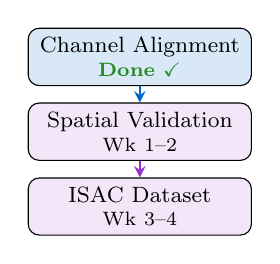
\begin{tikzpicture}[>=stealth, font=\footnotesize, node distance=0.6cm]
  \node[draw, rounded corners, fill=accent!15, text width=2.6cm, align=center] (a) {Channel Alignment\\[-1pt]\scriptsize\color{good}\textbf{Done \checkmark}};
  \node[draw, rounded corners, fill=plan!12, text width=2.6cm, align=center, below of=a, yshift=-0.35cm] (b) {Spatial Validation\\[-1pt]\scriptsize Wk 1--2};
  \node[draw, rounded corners, fill=plan!12, text width=2.6cm, align=center, below of=b, yshift=-0.35cm] (c) {ISAC Dataset\\[-1pt]\scriptsize Wk 3--4};
  \draw[->, thick, accent] (a) -- (b);
  \draw[->, thick, plan] (b) -- (c);
\end{tikzpicture}
\end{center}

\end{minipage}

\end{frame}

\end{document}
